\section{Pure approach}
\subsection{General}
\subsubsection{Performance}
Ground truth vs. pure, commission, image quantity 

The workers motivate their votes as follows: 
\begin{itemize}
	\item Higher value of information 
	\item Professionalism 
	\item Hidden information are given (e.g. size of the cleats, size of the smartphone storage) 
	\item The description is clear, short and to the point 
	\item Authenticity of the article 
	\item Grammatical issues 
\end{itemize}

\subsection{Title}
Correct format, 
The workers justify their selections of a title as follows: 
\begin{itemize}
	\item Amount of details 
	\item Attracts more attention 
	\item Research on eBay produces better results for the title 
	\item Experiences with online auctions 
	\item Wrong information 
	\item Too long 
\end{itemize}

\subsection{Description}
Description lengths Pure, commission, quantity 
Non-branded item 

\subsection{Category}

\subsection{Price Estimation}
RMSE formula 
Under/Over estimations 
Market price 

\subsection{Variations}
\subsubsection{Commission }
The ground truth items 1 and 3 received a majority of the votes from the crowd. The commissions were paid manually using the web interface of the Amazon Mechanical Turk web service. The value of the bonus has to be shortened to two digits after the point and rounded up to \$0.01, because of some restrictions of MTurk. The bonus aggregates to \$1.48 for both auctions. The worker received also an additional message: \\
''Dear worker, \\

You receive a commission (0.25\% of the end price) as bonus payment for your work. The end price of the eBay online auction was \$27.''
\begin{table}[h!]
	\begin{center}
	\begin{tabular}{| p{1cm} | p{1.5cm} | p{3cm} | p{1.5cm} | p{1.5cm} | p{3.5cm} |}
		\hline
		Ground truth number & End price (USD) & Task & Percentage & Bonus (USD) & Worker ID \\
		\hline
		1 & 4.99 & Title (Finding) & 0.25\% & 0.01 & A3HE1W5T6QO03X \\
		\hline
		1 & 4.99 & Title (Voting) & 0.1\% & 0.01 & A3N7O1NOBGX6U7 \\
		\hline
		1 & 4.99 & Title (Voting) & 0.1\% & 0.01 & A1DK26QAO4OOMQ \\
		\hline
		1 & 4.99 & Description (Improving) & 1\% & 0.05 & A2Y9ZNZ0F24GHB \\
		\hline
		1 & 4.99 & Description (Voting) & 0.05\% & 0.01 & A2FF8HA1OWKS83 \\
		\hline
		1 & 4.99 & Description (Voting) & 0.05\% & 0.01 & AJAOE1PSNKGUE \\
		\hline
		1 & 4.99 & Category & 0.25\% & 0.01 & A2ZT4MTMEVSLB9 \\
		\hline
		1 & 4.99 & Category & 0.25\% & 0.01 & A220ED0LJITW5I \\
		\hline
		1 & 4.99 & Category & 0.25\% & 0.01 & A2V8WJXA0USMZ \\
		\hline
		1 & 4.99 & Price & 0.5\% & 0.02 & A3L99RGPK6FZGH \\
		\hline
		3 & 27 & Title (Finding) & 0.25\% & 0.06 & A23BCMQN9ZU97B \\
		\hline
		3 & 27 & Title (Voting) & 0.1\% & 0.02 & A3N7O1NOBGX6U7 \\
		\hline
		3 & 27 & Title (Voting) & 0.1\% & 0.02 & A3I4BYP4DUC475 \\
		\hline
		3 & 27 & Description (Improving) & 1\% & 0.27 & A1IA4CST74I1Q8 \\
		\hline
		3 & 27 & Description (Voting) & 0.05\% & 0.01 & A3K77RSYXLLUQL \\
		\hline
		3 & 27 & Description (Voting) & 0.05\% & 0.01 & A25F7BNXEN8I5X \\
		\hline
		3 & 27 & Category & 0.25\% & 0.06 & A2ZT4MTMEVSLB9 \\
		\hline
		3 & 27 & Category & 0.25\% & 0.06 & A220ED0LJITW5I \\
		\hline
		3 & 27 & Category & 0.25\% & 0.06 & A2V8WJXA0USMZ \\
		\hline
		3 & 27 & Price & 0.5\% & 0.13 & A3L99RGPK6FZGH \\
		\hline
	\end{tabular}
	\end{center}
	\caption{}
\end{table}



 

\section{Hybrid approach}
The Random Forest approach shows the best performance over all three item categories independent of classification or regression (Figure). The accuracy of the classifier depends also on the item category. The RFC assign every third input to the right Sony Playstation price class. The plot of the mean absolute error (MAE, Figure) assured the strength of the classifier and visualise how far away the predictions are in average. kNN has an error of about four classes for the iPhone category, one class has a range of 25 USD. The comparison between the human-based and the machine-based prediction indicates that the crowd can't be as accurate as a machine. The lowest RMSE of the ground truth item number 2 (Apple iPhone) is \$76.32. Two machine learning algorithms have a smaller error (Figure). 
The normalised confusion matrix (Figure) of the iPhone classifiers illustrates the distribution of the assignments. The origin is located at the left top position, the x-axis represents the truth-values and the y-axis the values assigned by the classifier. The values were normalised per row. A perfect classifier would produce a diagonal which contains only ones. 
The scatter plot (Figure) is another way to visualise the relations between the truth and predicted values. The criteria of a perfect classifier are the same as for the confusion matrix. 
The same plots for the other categories and the exact accuracies/RMSEs/MAEs are enumerated in the appendix section (Reference).
\begin{figure}
\centering
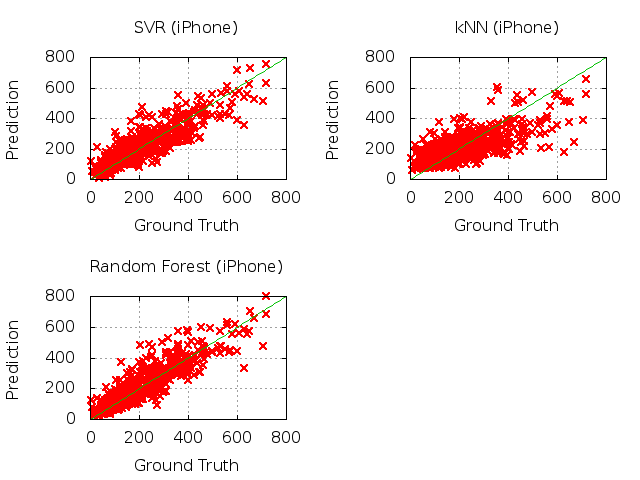
\includegraphics[scale=0.55]{images/plots/machine_learning/iphone/true_pred_iphone.png}
\caption{Scatter plot truth vs. prediction (iPhone)}
\label{truth_predict_iphone}
\end{figure}
\begin{figure}
\centering
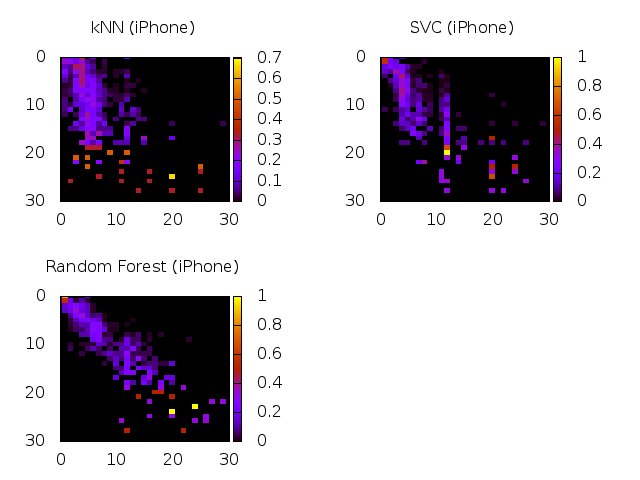
\includegraphics[scale=0.55]{images/plots/machine_learning/iphone/conf_mat_iphone.png}
\caption{Time/Error Function}
\label{crowdsourcing_desc_length}
\end{figure}

\begin{figure}
\centering
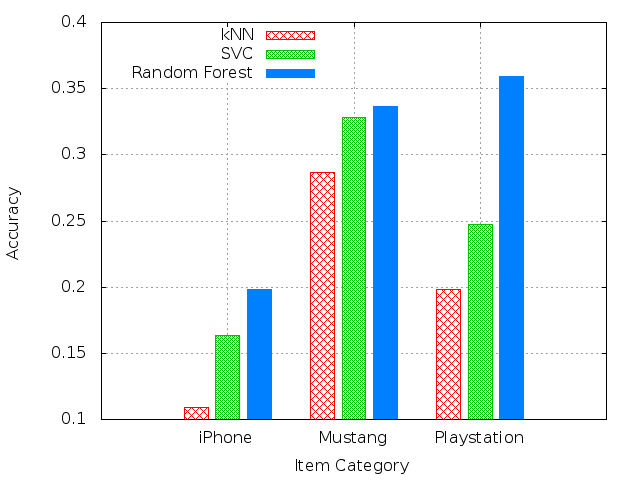
\includegraphics[scale=0.55]{images/plots/machine_learning/plot_price_classification_acc.png}
\caption{Time/Error Function}
\label{crowdsourcing_desc_length}
\end{figure}
\begin{figure}
\centering
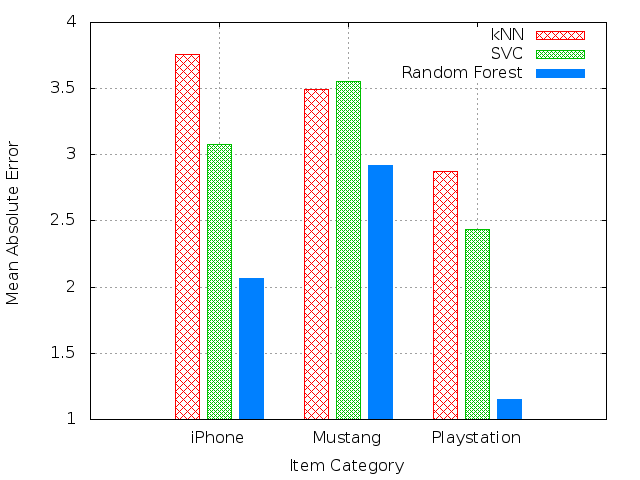
\includegraphics[scale=0.55]{images/plots/machine_learning/plot_price_classification_mae.png}
\caption{Time/Error Function}
\label{crowdsourcing_desc_length}
\end{figure}

\begin{figure}
\centering
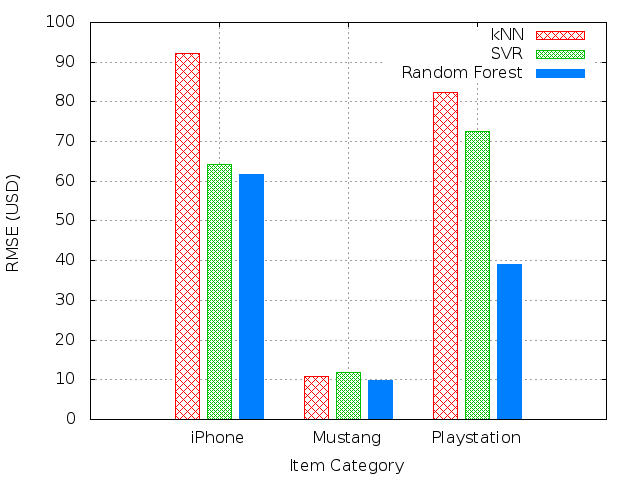
\includegraphics[scale=0.55]{images/plots/machine_learning/plot_price_regression_rmse.png}
\caption{Time/Error Function}
\label{crowdsourcing_desc_length}
\end{figure}


\begin{figure}
\centering
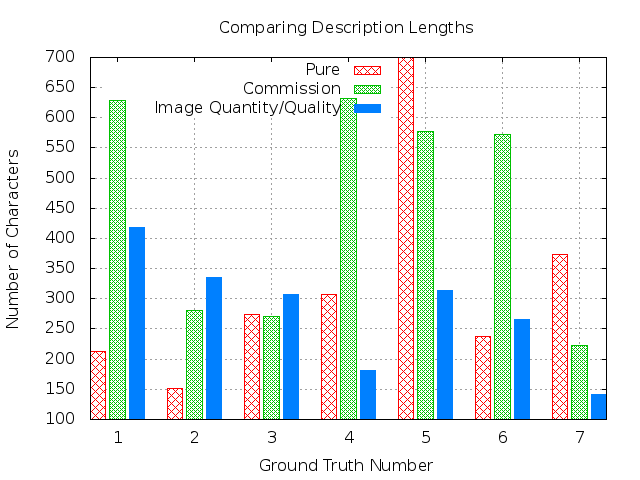
\includegraphics[scale=0.55]{images/plots/crowdsourcing/plot_description_length.png}
\caption{Evaluation of Description Lengths}
\label{crowdsourcing_desc_length}
\end{figure}
\begin{figure}
\centering
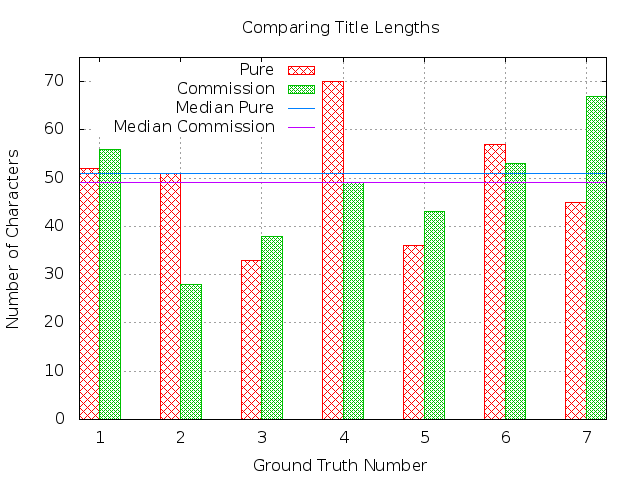
\includegraphics[scale=0.55]{images/plots/crowdsourcing/plot_title_length.png}
\caption{Evaluation of Title Lengths}
\label{crowdsourcing_desc_length}
\end{figure}
\begin{figure}
\centering
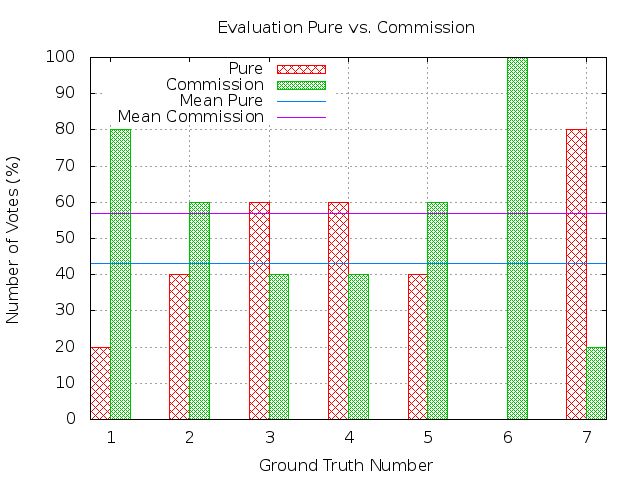
\includegraphics[scale=0.55]{images/plots/crowdsourcing/plot_evaluation_pure_vs_commission.png}
\caption{Evaluation of Pure vs. Commission}
\label{crowdsourcing_desc_length}
\end{figure}
\begin{figure}
\centering
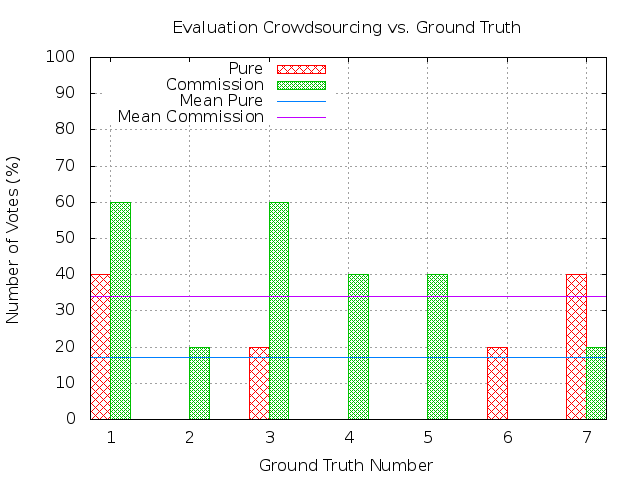
\includegraphics[scale=0.55]{images/plots/crowdsourcing/plot_evaluation_ground_vs_crowd.png}
\caption{Evaluation of Ground Truth vs. Crowdsourcing}
\label{crowdsourcing_desc_length}
\end{figure}
\begin{figure}
\centering
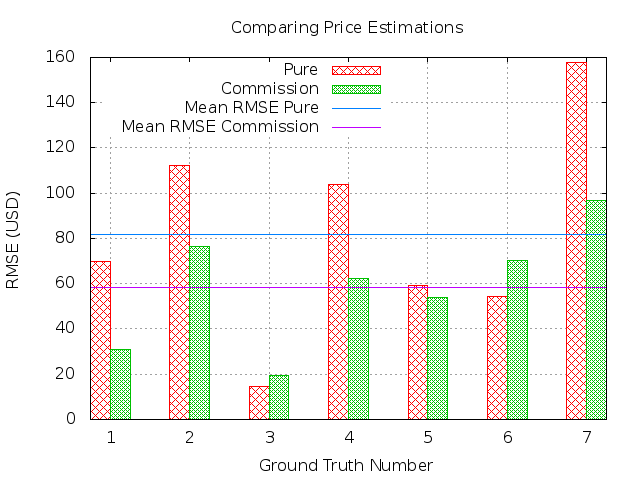
\includegraphics[scale=0.55]{images/plots/crowdsourcing/plot_price_rmse.png}
\caption{Price Prediction Quality}
\label{crowdsourcing_desc_length}
\end{figure}
\begin{figure}
\centering
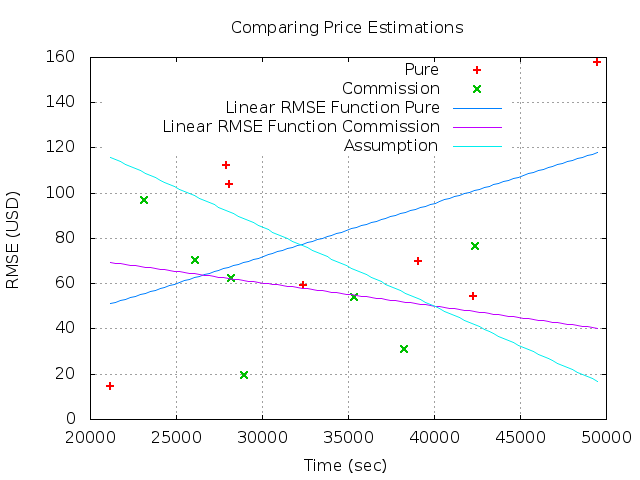
\includegraphics[scale=0.55]{images/plots/crowdsourcing/plot_time_rmse.png}
\caption{Time/Error Function}
\label{crowdsourcing_desc_length}
\end{figure}

